\documentclass[11pt]{article}
\usepackage{graphicx}
\input def.tex
\begin{document}
%EDIT THIS FILE AND FILL IN THE RELEVANT DETAILS.
\input hct_title.tex

%ENTER CYCLE APPLYING FOR (No. & PERIOD); ENTER DATE OF PROPOSAL SUBMISSION
{\bf Cycle applying for:}~~~~~~~\hfil Date: \hfil\\
%
%ENTER TITLE OF PROPOSAL AFTER CURLY BRACKETS
%
\\
{\bf 1. Title of the proposal : Late time emission of SN2014J, optical and Near Infrared observations } 

%IN THE FOLLOWING, CHANGE "NO" to "YES" WHERE APPLICABLE.
%
\NO~Short term \hfil \NO~Long term \hfil Number of cycles/nights:~~~~\hfil\\
\NO~Ongoing proposal \hfil Previous proposal code(s):~~~~~~~~~~~~~\hfil~~~~\\
\YES~Thesis topic \hfil Expected year of thesis submission: 2016  \hfil~~~\\
{\bf \small {If proposal is intended to support a Ph.\ D.\ project, please
include, in addition to the Scientific Justification, a brief outline of the 
Ph.\ D.\ project and the relevance of the proposal to the Ph.\ D.\ project}}\\

%
%LIST NAMES OF PROPOSERS WITH E-MAIL ADDRESS.
%
{\bf 2. List of Proposers: } {\sl indicate PI(s)}\\[1mm]
\begin{tabular}{|p{2in}|p{2in}|p{1.5in}|p{0.8in}|}
\hline
Proposer & Affiliation & e-mail & Will be present for observations?\\
\hline
 B. Leibundgut & ESO &bleibund@eso.org & \\ \hline
 S. Dhawan& ESO & sdhawan@eso.org& \\ \hline
S. Taubenberger & ESO & tauben@mpa-garching.mpg.de & \\ \hline
W. Kerzendorf & ESO & wkerzend@eso.org & \\ \hline
K. Maguire & ESO & maguirek@eso.org & \\ \hline
J. Spyromilio & ESO & jspyromi@eso.org & \\ \hline
\end{tabular}

%NAME AND ADDRESS OF PROPOSER FOR CONTACT
%
{\bf 3. Contact Name \& Address: }\\
European Southern Observatory,
Karl Schwardschild Strasse, 2
Garching bei M�nchen, 85748, 
Germany
\\
\\
\\
Telephone:\\
Fax:\\

%GIVE A BRIEF ABSTRACT OF THE PROPOSAL
%
\textbf{ 4. Abstract: }
Type Ia supernovae (SNe Ia) are thermonuclear explosions of white dwarfs (WDs) in binary systems. Detailed observations of large samples have displayed a heterogeneity in the properties of SNe Ia near maximum light. The late phases in the life of an SN offer a different opportunity to study the physics of the ejecta and are potent in distinguishing between different explosion models. 
In this proposal, we aim to observe SN2014J, a nearby SN in M82, at very late phases in the optical and NIR. Since, at such late phases, the $\gamma$-ray escape fraction is much higher than at maximum, hence, most of the energy is deposited by the positrons. Thus, we can discern the nature of the magnetic field using the positron escape fraction. Probing the occurrence of an Infrared Catastrophe at these epochs allows us to understand the ejecta temperature and density distribution. Since most observations of SNeIa in the NIR only extend to $\sim$ +700, observations at even later phases offer an interesting prospect to learn about the physics of SNeIa.
\\ 
%BEGIN ABSTRACT
\\
\\
\\
\\
\\
\\
\\
\\
\\
\\
\\
%END ABSTRACT

%\newpage 
{\it HCT Proposal}\hskip 5cm {\it Page 2} \hfill {\it Cover page (contd)}\\[1mm]
\hrule

{\bf 5. Status of ongoing / previous proposals:}\\ 
%FIRST TIME APPLICANTS MAY ENTER `NA'
{\sl \small {1. Please give a brief status report of any previous HCT proposals, and
attach any preprint/reprint based on these HCT observations\\
2. If your proposal is long-term / on-going, briefly state the status of the
proposal, mentioning the progress with respect to the science goals.}}\\
{\bf \small {NOTE: Incomplete proposals are likely to be given low priority
or rejected}
}
\\
N/A
\\
\\
\\
\\
\\
\\
\\
\\
\\
\\
\\
\\
\\
\\
\\
\\
\\
\\
\\
\\
\\


\hrule
{\bf For official purpose only}

{\it Referee's comments:}\\
\\
\\
\\
\\
\\
\\
\\
\\
{\it Science feasibility:} \hfil {\it Technical feasibility:} \hfil \\

{\it Grade of the proposal:} \hfil \\

{\it Dates allotted:}

\newpage
{\it HCT Proposal}\hskip 5cm {\it Page 3} \hfill {\it Observing Details}\\[1mm]
\hrule
{\bf 6. Scheduling request: }~~~~~\\
%
%IN THE FOLLOWING LINES, CHANGE "NO" to "YES" TO INDICATE THE DESIRED 
%SCHEDULING REQUEST 

\YES~Dark night is essential \hfil \NO~Grey night is all right~~~~~\\
\NO~Bright night is all right \hfil \NO~Time-critical observations\\
\NO~Target of Opportunity \hfil \NO~Other (specify) ~~~~~~~~~~~~~\\

\begin{tabular}[t]{p{9cm}p{9cm}}
{No. of nights requested: 0.5 }(total exposure time and calculations in section \textbf{10})\\
{Preferred dates: None} & {Impossible dates: June 30 to August 31}\\
 & \\
 & \\
 & \\
 & \\
\end{tabular} \\ 

{\bf 7. Justification for scheduling request: }\\
SN2014J has the lowest visibility between end of June and end September. 

We request dark nights since they significantly reduce exposure times in the optical. With a dark + 1 mag sky brightness, the exposure times are great by a factor of 5. 
We would like to observe the SN in $1.5^{"}$ or better seeing. 
\\
\\
\\
\\
{\bf 8. Instrument:} {\sl check all that apply}\\
%
% IN THE FOLLOWING LINES, CHANGE "NO" to "YES" TO INDICATE THE REQUIRED
% INSTRUMENT(S)
\YES~HFOSC\\
\NO~Optical CCD Imager\\
\YES~TIFR Near-IR Spectrometer (TIRSPEC)\\[1mm]

{\bf 9. Mode of Observation:} {\sl check all that apply}\\ 
%
% IN THE FOLLOWING LINES, CHANGE "NO" to "YES" TO SPECIFY THE MODE(S) OF
% OBSERVATION
\YES~Imaging
\NO~Spectroscopy
\\[2mm]

{\bf 10. Brief description of observations: } \\
We request observations of the target at intervals of 30 days, starting from the first epoch in May. For each observation date, we would like to observe the SN in the  B to K filters with the HFOSC(BVRI) and TIRSPEC (JHK) instruments  \\


the total number of observations requested is 2 epochs. \\

To calculate the exposures in the optical, we normalise the maximum light observations of SN2001el (a well-observed normal Ia) to the peak of SN2014J in the $BVRI$ filters. As a result, we use the predicted fading of SN2001el to get the magnitudes at these late phases. 
We summarise the exposure times in  table \ref{tab:exp}
Note: we use the Liverpool Telescope's exposure time calculator to get these estimates 
\begin{tabular}{llll|}
\\
\hline
Filter & Magnitude & Exposure (s; dark, $1.5^{"}$)  & Exposure (s; dark + 1 mag, $1.5^{"}$) \\
\hline
B	& 21.31   & 480 & 1200\\
V	& 20.31 & 200 & 400\\
R	&  20.61	&  300  & 650\\
I	&   17.99  & 60 &   60\\
\hline
\label{tab:exp}
\end{tabular}
\newpage
Hence, the total time for each epoch in the optical will be 40 mins. Including a conservative estimate of overheads, we request 1 hour of observations in the optical at each epoch. 

For  calculations in the infrared we use the TIRSPEC exposure time calculator. For our desired signal to noise, we require 5 dithers of 6 frames with 15s exposures. Since, we require off source images for sky subtraction, we would like to split this observation into two sequences of 5 dithers with 3 frames. 
Hence, we would obtain a total exposure time of 450s 
We multiply this by a factor of 3 to get the overheads for the on-source and off-source sequences. Hence, the total time in each filter for the observation will be close to 25 minutes. Thus, we require 1.5 hours for each epoch.

The total time for each epoch, optical + IR is 2.5 hours.
 Hence, the total time requested for the semester is 2 X 2.5 = 5 hours. 
\\
\\
\\
\\
{\bf 11. Plans for data reduction and analysis: }
We plan to use the available reduction software for TIRSPEC and HFOSC to reduce the images .
We have downloaded the photometry templates for M82 for accurate host galaxy subtraction. 
We currently have routines ready for the bolometric light curve calculation which have also been testing on data for other projects. 
 \\


%\newpage
{\it HCT Proposal}\hskip 5cm {\it Page 4} \hfill {\it Observing Details (contd)}\\[1mm]
\hrule
{\bf 12. Instrument Resource Requirements:}\\[1mm]
% IN THE FOLLOWING LINES, CHANGE "NO" to "YES" TO INDICATE THE REQUIREMENT(S).

{\bf HFOSC}\\
{\bfs Broad Band Filters:} \NO~U \YES~B \YES~V \YES~R \YES~I \NO~I$_c$ 
\NO~$z$\\ [1mm]
%{\bfs Narrow Band Filters:} \NO~486.1(10) \NO~500.7(10) \NO~656.3(10) 
%\NO~672.4(10) \NO~656.3(50) \\[1mm]
%{\bfs Grisms:} \NO~Gr.5 \NO~Gr.7 \NO~Gr.8 \NO~Gr.9 \NO~Gr.10 \NO~Gr.11
%\NO~Gr.12 \NO~Gr.14 \NO~Gr.15 \NO~Gr.17\\[1mm]
%{\bfs Slits:} \NO~67(s) \NO~67(l) \NO~100(m) \NO~100(l) \NO~134(s) 
%\NO~134(l) \NO~167(l) \NO~335(l) \NO~1340(l)\\[1mm]
\iffalse
{\bf Optical CCD Imager}\\ 
{\bfs Broad Band Filters:} \NO~U \NO~B \NO~V \NO~R \NO~I \NO~I$_c$ 
\NO~$z$\\[1mm]
{\bfs Narrow Band Filters:} \NO~372.7(5) \NO~486.1(5) \NO~500.7(5) 
\NO~656.3(5) \NO~664.3(10) \NO~672.4(10) \NO~680.4(10) \NO~688.4(10) 
\NO~696.4(10) \NO~704.4(10) \NO~712.4(10)\\[1mm]
\fi
{\bf TIRSPEC}\\
{\bfs Broad Band Filters:} \YES~J \YES~H \YES~K$_{\rm s}$ \\ [1mm]
%{\bfs Narrow Band Filters:} \NO~Methane off (1.584, 3.6\%) \NO~[Fe II] (1.645, 1.6\%) \NO~Methane on (1.654, 4.0\%)
%\NO~H2(1-0) (2.1239, 2.0\%) \NO~Br$\gamma$ (2.166, 0.98\%) \NO~K-cont (2.273, 1.73\%) \NO~CO(2-0) (2.287, 1.33\%) \\[1mm]
%{\bfs Single Order Dispersers:} \NO~Y (1.02--1.20) \NO~J (1.21--1.48) \NO~H (1.49--1.78) \NO~K (2.04--2.35)\\[1mm]
%{\bfs Cross Dispersers:} \NO~YJ (1.02--1.49) \NO~HK (1.50--2.45)\\[1mm]
%{\bfs Slits:} \NO~1"(s) \NO~1"(l), \NO~1.5"(s) \NO~1.5"(l) \NO~2"(s)
%\NO~2"(l) \NO~3"(s) \NO~3"(l) \NO~8"(s) \NO~8"(l)\\[1mm]

% LIST THE OBJECTS PROPOSED TO BE OBSERVED BELOW. PLEASE NOTE THAT THE PROPOSAL
% MAY BE REJECTED IF NO LIST IS PROVIDED.
%

{\bf 13. List of objects: (essential)}\\

\begin{tabular}{|p{1in}|p{1.5in}|p{1.5in}|p{0.5in}|p{0.5in}|p{0.5in}|}
\hline
Name & RA (hh mm ss)& Dec (dd mm ss) & Epoch & $V$ mag & size$^*$ \\
\hline
SN2014J & 09 55 42.12 & +69 40 25.9  &  J2000 & 20.31 &  N/A  \\\hline
\hline
 \multicolumn{6}{l}{*for extended objects}\\
\end{tabular}

\newpage
{\it HCT Proposal}\hskip 5cm {\it Page 5} \hfill {\it Scientific Justification}\\[1mm]
\hrule
{\bf 14. Scientific Justification:} {\sl Type Ia supernovae (SNe~Ia) are thermonuclear explosions of white dwarfs in a binary system. Their use as distance indicators in cosmology has led to dedicated efforts to obtain data for large samples of SNeIa. This has revealed a heterogeneity in the photometric and spectroscopic properties of the explosions. However, most of the assimilated data for the SNe~Ia are directed towards understanding them during the early photospheric phase. At late phases, the $\gamma$ ray escape fraction increases and most of the light curve is powered by the positrons. Hence, these late-phases of these SNe offer other opportunities to study the physics of these explosions, for eg. constraining the geometry of the magnetic field.

At phases greater than $\sim$ 200 days past maximum light, the light curves are powered by the deposition of positron kinetic energy. The fraction of positron energy deposited into the ejecta is thought to depend on the magnetic field configuration, with a stronger magnetic field leading to higher fraction of positrons being trapped. Thus, the late-time (pseudo-)bolometric light curve (integrated from filters B to K) is an efficient tool in constraining the configuration of the magnetic field in the SNe and, in principle can constrain the contribution these positrons make to the galactic 511 keV line.  In figure \ref{fig:bol}, we can see the (pseudo-)bolometric light curve for SN2001el from Stritzinger $\&$ Sollerman 2007, compared to their toy model. Their bolometric light curve only extends out to $\sim$  +440 days.

A few recent studies have shown that SNeIa show a flattening of the Near Infrared (NIR) light curve at a few hundred days past maximum light . This is attributed to a flux redistribution at late epochs from the optical to the NIR. However, there objects with such late time data have very sparse sampling and no coverage beyond $\sim$ +700 days. 

SN2014J, the nearest supernova in the past 4 decades provides a unique laboratory to study this late time behaviour. Dedicated near-maximum observations have led to epochal discoveries, like the first observation of the $^{56}Co$ line in the $\gamma$ rays.  Its proximity means that it is bright, even at late epochs $\geq$ +700 days, which allows us to probe the physics of the explosion out to later epochs than current studies. A time sampling of observations every $\sim$ 30-50 days within the range of +300-+800 days would allow us to constrain the evolutionary behaviour  of this late time decline in the NIR precisely. This would be the first set of well-sampled observations of an SNIa in the mentioned phase range. Observations post +700 days will allow us to observe the behaviour of SNeIa in the NIR at very late epochs, to constrain when the flattening ends and what the nature of the light curve is at $>$ +700 days. 

At late times, the exponential decline in the heating due to radioactive decay and the flattening of the cooling curve lead to a dramatic ionisation shift such that only the ground state levels are populated. This leads to a significant decrease in the flux in the optical and NIR filters, with most of the emission dominated in the mid-IR region. This is known as the the Infrared Catastrophe (IRC; Axelrod 1980). Theoretical models  (Milne et al. [2001]) predict an IRC to occur at $\sim$ +500 days. Observations of SN2001el at late times do not show any signatures of an IRC. However, due to sparse sampling at these epochs, one cannot exclude the possibility of an IRC having occurred during the epochs where the SN wasn't observed. A similar difficulty exists for SN2003hv (Leloudas et al. [2009]). Hence, a good sampling at such late times is crucial to discerning the presence of an IRC, and therefore, the physical conditions in the ejecta. 

%Very late time optical and NIR observations  allow constraints on the occurrence of an IRC in the ejecta. The IRC is expected to occur once the ejecta temperature drops below a threshold. For SN2003hv, it has been seen that there in no drop in luminosity in the NIR which suggests that at least part of the ejecta is above the temperature threshold. Observations with regular time sampling in the phase range between +550 and  +800 days will allow strong constraints on the occurrence of an IRC in 2014J. An absence of the IRC in the given phase range can be explained by the clumping of the ejecta in particular regions, which would postpone the onset of the IRC. Since there are no observations at phases $>$ +700 days, the phase range of +700 to +800 days offers a new window into constraining the presence of an IRC. 
\section*{References}
\iffalse
%\begin{thebibliography}{99}
\bibitem{Axelrod80} 
Axelrod T.~S., 1980, PhDT 

\bibitem[\protect\citeauthoryear{Kerzendorf et 
al.}{2014}]{K14} Kerzendorf W.~E., Taubenberger S., 
Seitenzahl I.~R., Ruiter A.~J., 2014, ApJ, 796, LL26


\bibitem[\protect\citeauthoryear{Leloudas et 
al.}{2009}]{2009A&A...505..265L} Leloudas G., et al., 2009, A\&A, 505, 265 

\bibitem[\protect\citeauthoryear{Milne, The, 
\& Leising}{2001}]Milne P.~A., The L.-S., Leising M.~D., 2001, ApJ, 559, 1019 



\bibitem[\protect\citeauthoryear{Taubenberger et 
al.}{2015}]{T15} Taubenberger S., et al., 2015, MNRAS, 448, 
L48 

%\end{thebibliography}
\fi


\newpage
{\bf 14a. PhD project Outline:}
This proposal is intended to support part of a PhD project. The focus of the project is to understand the Near Infrared behaviour of Type Ia supernovae, with an emphasis on late time behaviour. 
The Near Infrared offers complementary information to the optical for understanding the physical processes in Type Ia SNe. They appear to be more uniform at longer wavelength with a scatter $< $ 0.2 mag. Another, very interesting feature in the NIR light curves is the appearance of a second maximum, around 2 weeks after maximum light in $B$-band. We investigated the relation between the second maximum (specifically the timing, termed as $t_2$). We found correlations between $t_2$ and the optical decline rate ($\Delta m_{15}$). We also find that the $t_2$ is related very strongly to the post-maximum colour evolution in the optical. These correlations point to a common origin of this diversity from the large range of $^{56}Ni$ produced in the SNe. Hence, the NIR light curve at $\sim$ 2 - 3 weeks post maximum is a probe of the total radioactive nickel synthesised in the ejecta. 

In the transitional phase (a few months after maximum light), the SN is getting progressively more transparent to the $\gamma$ rays and the light curve has an increasing contribution from positrons. Along with our conducted study of the second maximum, we would like to understand the nature of the SN when it is in its nebular phase. At these phases, we can probe the inner regions of the ejecta. While line profile measurements from spectroscopy can shed light on the ejecta distribution, the photometric measurements at $>$ +200 days are key in uncovering global parameters of the ejecta. 

Observations of a handful of SNe in the JHK bands show a flattening of the decline in the NIR. However, since these SNe are significantly farther and fainter  than SN2014J (for e.g. SN2001el is $\sim $3 magnitudes than SN2014J) there is sparse sampling at late times. Thus,  for part of the PhD, we would like to analyse well-sampled data of SN2014J in the nebular phase.
 } 
\newpage

\begin{figure}
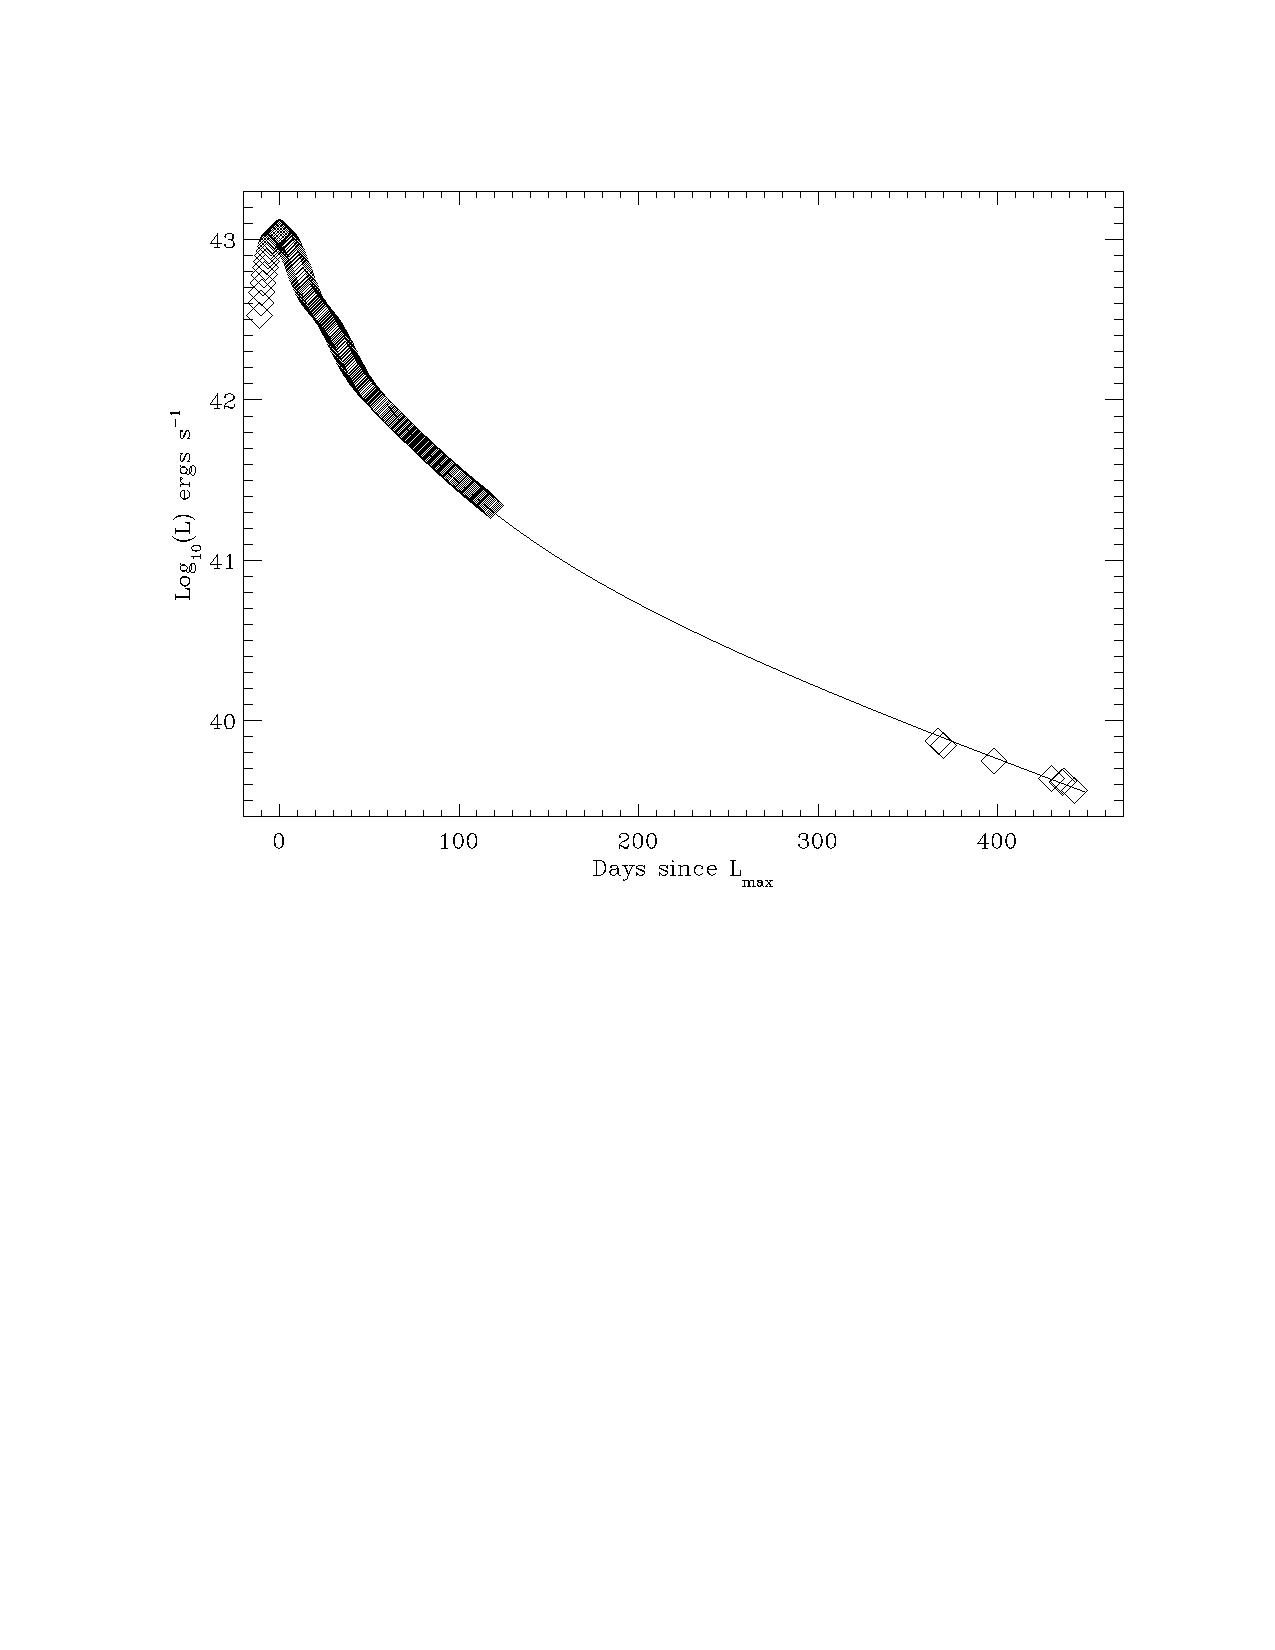
\includegraphics[width=.8\textwidth, trim=0 300 60 0]{sn01el_bol.pdf}
\caption{(Pseudo-) bolometric light curve of SN2001el from Stritzinger $\&$ Sollerman 2007}
\end{figure}

\begin{figure}
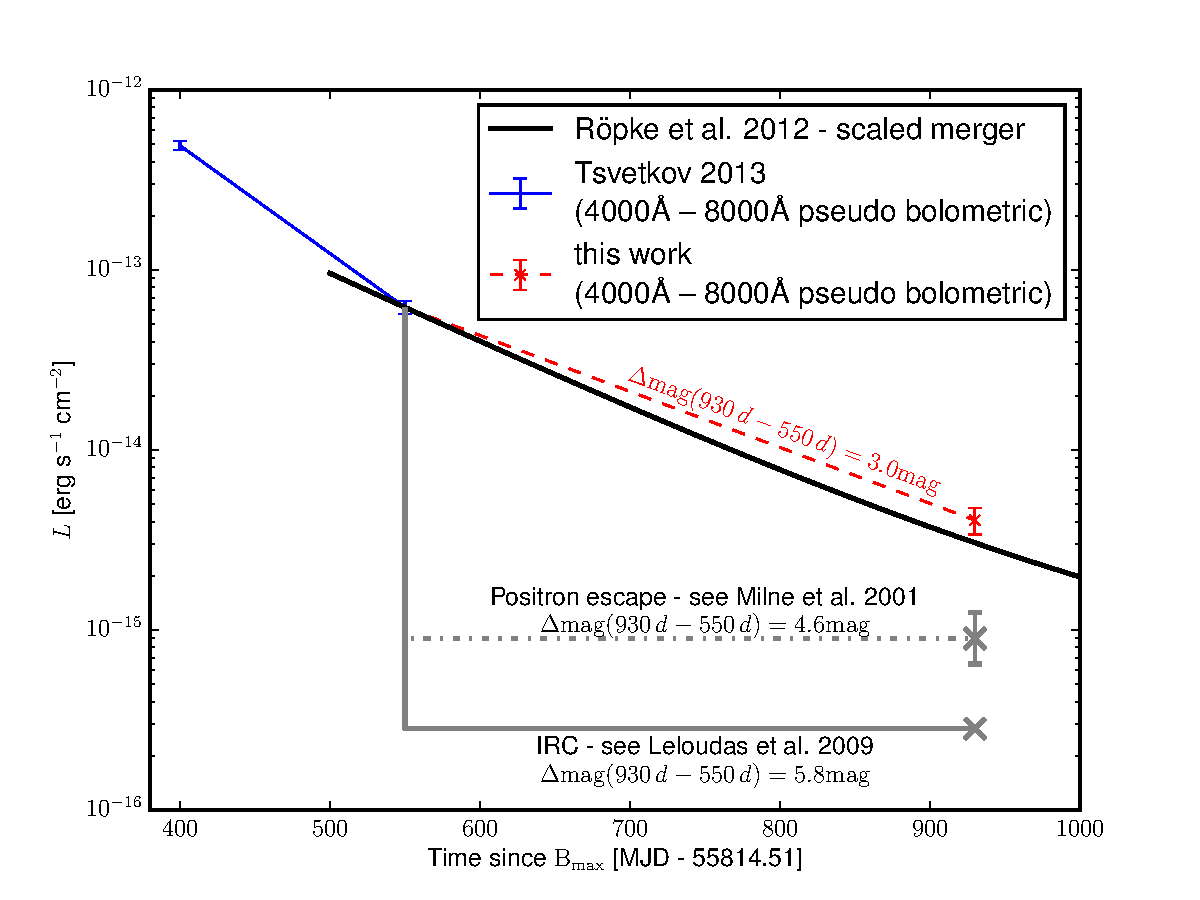
\includegraphics[width=\textwidth, trim=0 0 30 0]{sn11fe_bolom.pdf}
\caption{The (pseudo-) late time light curve of SN2011fe (Kerzendorf et al. [2014]. Although model predictions expect an IRC, there is no evidence in the observations for the presence of an IRC. }%Light curve of SN2001el in u - K filters (Stritzinger $\&$ Sollerman 2007). The flattening of the light curve can be seen in the JHK filters.}
\end{figure}
\end{document}
